\documentclass[conference]{IEEEtran}
\IEEEoverridecommandlockouts
\usepackage{cite}
\usepackage{amsmath,amssymb,amsfonts}
\usepackage{graphicx}
\graphicspath{{../plots_and_table/Generated/}}
\usepackage{textcomp}
\usepackage{hyperref}
\usepackage{xcolor}
\usepackage{booktabs}
\usepackage{multirow}
\usepackage{placeins}
\usepackage{float}
\usepackage{tikz}
\usepackage{balance}
\usepackage{stfloats}
\usepackage{caption}
\usepackage{adjustbox}
\usepackage{array}
\usepackage{titlesec}
\titlespacing*{\section}{0pt}{0.45em}{0.25em}
\titlespacing*{\subsection}{0pt}{0.35em}{0.15em}
\newcolumntype{L}[1]{>{\raggedright\arraybackslash}p{#1}}
\usetikzlibrary{arrows.meta,backgrounds,fit,positioning,shapes.geometric,calc}

\begin{document}
	
	\title{Towards Practical On-Device Android Malware Detection via Lightweight Static Analysis}
	
	\author{\IEEEauthorblockN{Abdullah Faiyaz}
		\IEEEauthorblockA{\textit{Department of CSE,}
			\textit{BUET}\\
			2005065@ugrad.cse.buet.ac.bd}
		\and
		\IEEEauthorblockN{Jarin Tasnim}
		\IEEEauthorblockA{\textit{Department of CSE,}
			\textit{BUET}\\
			2005083@ugrad.cse.buet.ac.bd}
		\and
		\IEEEauthorblockN{Mohammad Sadnam Faiyaz}
		\IEEEauthorblockA{\textit{Department of CSE,}
			\textit{BUET}\\
			2005111@ugrad.cse.buet.ac.bd}
		\and
		\and
		\IEEEauthorblockN{Md. Mostofa Akbar}
		\IEEEauthorblockA{\textit{Department of CSE,}
			\textit{BUET}\\
			mostofa@cse.buet.ac.bd}
	}
	
	\maketitle
	\vspace{-0.35em}
	
	\noindent\begin{minipage}[t]{0.485\textwidth}
		\footnotesize
		\noindent\textbf{Abstract---}\ignorespaces
		Android malware keeps growing, yet accurate detectors often depend on cloud backends or heavyweight analysis ill-suited to private, offline screening on commodity phones.
		We present \textbf{VigiDroid}, an on-device static pre-screener that orchestrates literature-derived lightweight models through ONNX Runtime without uploading APK data.
		Detectors are trained offline on a large temporal APK corpus, exported with train/serve parity checks, and deployed as verified bundles together with a calibrated cascade policy.
		On the phone, VigiDroid parses each APK once, runs a four-tier early-exit cascade, and logs per-stage resource metrics as append-only JSONL for thesis evaluation.
		\par\vspace{0.35em}
		\noindent\textbf{Index Terms---}\ %
		Android malware detection, static analysis, on-device inference, ONNX, ensemble learning, mobile security.
		\par\vspace{0.25em}
		
		\section{Introduction}
		Static malware analysis reports strong offline accuracy, yet few works optimize deployment on phones with limited CPU, memory, and battery.
		\textbf{VigiDroid} re-implements ten lightweight static detectors in ONNX and profiles accuracy alongside extraction cost on real hardware.
		\textbf{Dex+Broadcast fusion} reaches 97.0\% accuracy and F1 of 0.950 at 0.5\,ms mean stage time.
		\section{Background and Related Works}
		Android malware detection spans permission-based linear models~\cite{linregdroid}, MLDP feature selection~\cite{mldp}, broadcast-receiver mining~\cite{broadcast}, byte-level 1-D CNNs on APK tails~\cite{bytecnn}, and multi-branch DEX/manifest fusion inspired by MSFDroid~\cite{msfdroid}.
		SeqMobile~\cite{seqmobile} showed on-device RNN screening over permissions and API traces;
		SAMADroid~\cite{samadroid} combined lightweight local checks with cloud dynamic analysis, but modern Android privilege restrictions limit that pattern.
		DL-Droid~\cite{dldroid} executed apps on real hardware for dynamic labels, which is accurate yet impractical for routine offline screening.
		Overall, prior work achieves strong offline accuracy but rarely reports deployment-aware trade-offs on commodity phones.
		\section{Proposed Methodology}
		\textbf{PC model development (Fig.~\ref{fig:offline-workflow}).}
		Each detector follows an eight-phase pipeline (P0--P8): index a $\sim$500\,GB temporal APK corpus, extract features, train on 2020--2021 samples, evaluate on 2022--2023 holdout, export ONNX bundles with thresholds and vocabularies, and pass a parity gate ($\Delta p \leq 10^{-4}$) before any Android integration.
		\textbf{On-device system (Fig.~\ref{fig:vigidroid-app-flow}).}
		VigiDroid runs inference locally via ONNX Runtime, parses each APK once into a shared \texttt{FeatureContext}, executes a calibrated four-tier cascade with early exit, fuses tier scores into \texttt{benign}/\texttt{malware}/\texttt{uncertain} verdicts, and appends per-stage wall time, CPU, memory, and battery metrics to JSONL for thesis analysis.
	\end{minipage}\hfill
	\begin{minipage}[t]{0.485\textwidth}
		\vspace{0pt}
		\centering
		\adjustbox{max width=\linewidth, max totalheight=0.42\textheight, keepaspectratio, center}{%
			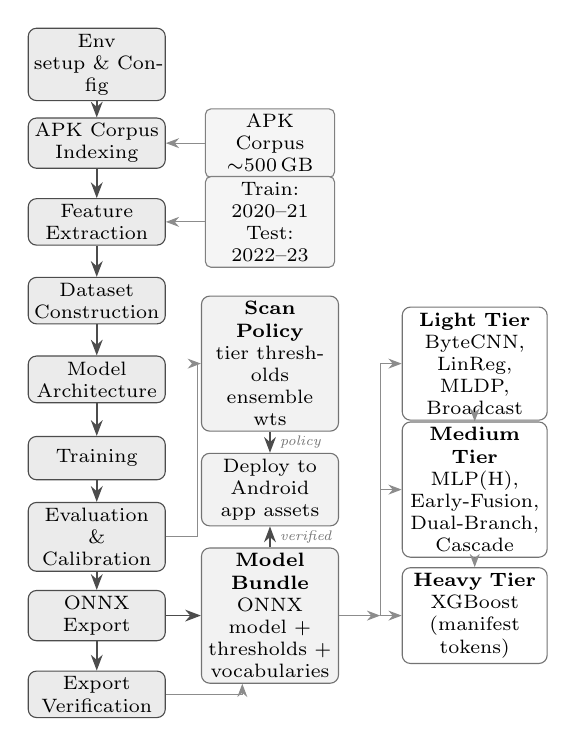
\begin{tikzpicture}[
				font=\scriptsize,
				>=Stealth,
				phase/.style={
					rectangle, rounded corners=3pt,
					draw=black!70, fill=black!8,
					text width=1.6cm, align=center,
					minimum height=0.55cm, inner sep=2pt
				},
				tierbox/.style={
					rectangle, rounded corners=3pt,
					draw=black!55, fill=white,
					text width=1.7cm, align=center,
					minimum height=0.55cm, inner sep=2pt
				},
				side/.style={
					rectangle, rounded corners=2pt,
					draw=black!50, fill=black!4,
					text width=1.5cm, align=center,
					minimum height=0.5cm, inner sep=2pt
				},
				mid/.style={
					rectangle, rounded corners=3pt,
					draw=black!55, fill=black!5,
					text width=1.6cm, align=center,
					minimum height=0.55cm, inner sep=2pt
				},
				arr/.style={->, semithick, black!70},
				sarr/.style={->, thin, black!45},
				lbl/.style={font=\tiny\itshape, black!55}
				]
				\node[phase] (setup) at (0,  0.0) {Env setup~\&~Config};
				\node[phase] (index) at (0, -1.0) {APK Corpus\\Indexing};
				\node[phase] (feat)  at (0, -2.0) {Feature\\Extraction};
				\node[phase] (load)  at (0, -3.0) {Dataset\\Construction};
				\node[phase] (arch)  at (0, -4.0) {Model\\Architecture};
				\node[phase] (train) at (0, -5.0) {Training};
				\node[phase] (eval)  at (0, -6.0) {Evaluation \&\\Calibration};
				\node[phase] (onnx)  at (0, -7.0) {ONNX\\Export};
				\node[phase] (parity)at (0, -8.0) {Export\\Verification};
				\foreach \a/\b in {setup/index, index/feat, feat/load, load/arch,
					arch/train, train/eval, eval/onnx, onnx/parity}
				\draw[arr] (\a) -- (\b);
				
				\node[side] (corpus) at (2.2, -1.0) {APK Corpus\\$\sim$500\,GB};
				\node[side] (split)  at (2.2, -2.0) {Train: 2020--21\\Test: 2022--23};
				\node[mid] (policy) at (2.2, -3.8) {\textbf{Scan Policy}\\tier thresholds\\ensemble wts};
				\node[mid] (phone) at (2.2, -5.4) {Deploy to\\Android\\app assets};
				\node[mid, minimum height=0.65cm] (bundle) at (2.2, -7.0) {\textbf{Model Bundle}\\ONNX model +\\thresholds +\\vocabularies};
				
				\draw[sarr] (corpus.west) -- (index.east);
				\draw[sarr] (split.west)  -- (feat.east);
				\draw[sarr] (eval.east) -- ++(0.4,0) |- (policy.west);
				\draw[arr] (onnx.east) -- (bundle.west);
				\draw[sarr] (parity.east) -| ([xshift=-10pt]bundle.south);
				\draw[arr] (policy.south) -- node[right, lbl] {policy} (phone.north);
				\draw[arr] (bundle.north) -- node[right, lbl] {verified} (phone.south);
				
				\node[tierbox] (tlight) at (4.8, -3.8) {\textbf{Light Tier}\\ByteCNN, LinReg,\\MLDP, Broadcast};
				\node[tierbox] (tmed) at (4.8, -5.4) {\textbf{Medium Tier}\\MLP(H), Early-Fusion,\\Dual-Branch, Cascade};
				\node[tierbox] (theavy) at (4.8, -7.0) {\textbf{Heavy Tier}\\XGBoost\\(manifest tokens)};
				\draw[draw=black!45, thin] (3.6, -3.8) -- (3.6, -7.0);
				\draw[sarr] (bundle.east) -- (3.6, -7.0);
				\draw[sarr] (3.6, -3.8) -- (tlight.west);
				\draw[sarr] (3.6, -5.4) -- (tmed.west);
				\draw[sarr] (3.6, -7.0) -- (theavy.west);
				\draw[sarr, densely dashed] (tlight.south) -- (tmed.north);
				\draw[sarr, densely dashed] (tmed.south) -- (theavy.north);
		\end{tikzpicture}}
		\captionof{figure}{Offline model development pipeline}
		\label{fig:offline-workflow}
		
		\vspace{0.8em}
		
		\adjustbox{max width=\linewidth, max totalheight=0.46\textheight, keepaspectratio, center}{%
			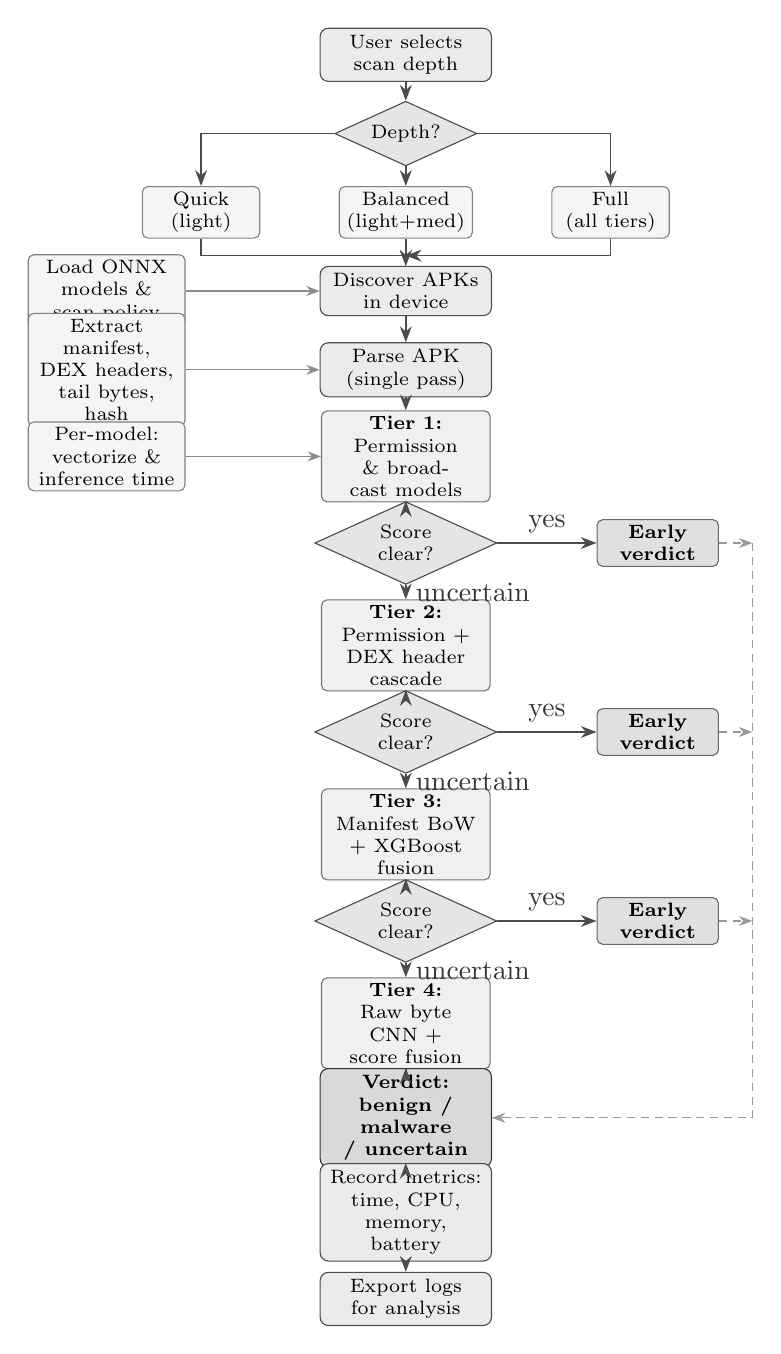
\begin{tikzpicture}[
				font=\scriptsize,
				>=Stealth,
				main/.style={
					rectangle, rounded corners=3pt,
					draw=black!70, fill=black!8,
					text width=2.0cm, align=center,
					minimum height=0.58cm, inner sep=2.5pt
				},
				decision/.style={
					diamond, aspect=2.2,
					draw=black!70, fill=black!10,
					text width=1.1cm, align=center,
					inner sep=1pt
				},
				verdict/.style={
					rectangle, rounded corners=3pt,
					draw=black!80, fill=black!15,
					text width=2.0cm, align=center,
					minimum height=0.55cm, inner sep=2.5pt,
					font=\scriptsize\bfseries
				},
				side/.style={
					rectangle, rounded corners=2pt,
					draw=black!50, fill=black!4,
					text width=1.85cm, align=center,
					minimum height=0.5cm, inner sep=2pt
				},
				tiernode/.style={
					rectangle, rounded corners=2pt,
					draw=black!55, fill=black!6,
					text width=2.0cm, align=center,
					minimum height=0.5cm, inner sep=2pt
				},
				exitnode/.style={
					rectangle, rounded corners=2pt,
					draw=black!60, fill=black!12,
					text width=1.4cm, align=center,
					minimum height=0.42cm, inner sep=2pt,
					font=\scriptsize\bfseries
				},
				arr/.style={->, semithick, black!70},
				sarr/.style={->, thin, black!45},
				darr/.style={->, densely dashed, thin, black!40},
				lbl/.style={font=\scriptsize, black!60}
				]
				\node[main] (ui) at (0, 0.0) {User selects\\scan depth};
				\node[decision] (depth) at (0, -1.0) {Depth?};
				\node[side, text width=1.35cm] (dq) at (-2.6, -2.0) {Quick\\(light)};
				\node[side, text width=1.55cm] (db) at ( 0.0, -2.0) {Balanced\\(light+med)};
				\node[side, text width=1.35cm] (df) at ( 2.6, -2.0) {Full\\(all tiers)};
				\draw[arr] (ui) -- (depth);
				\draw[arr] (depth.west) -| (dq.north);
				\draw[arr] (depth.south) -- (db.north);
				\draw[arr] (depth.east) -| (df.north);
				
				\node[main] (scan) at (0, -3.0) {Discover APKs\\in device};
				\draw[arr] (dq.south) -- (-2.6, -2.55) -- (0, -2.55) -- (scan.north);
				\draw[arr] (df.south) -- ( 2.6, -2.55) -- (0, -2.55);
				\draw[arr] (db.south) -- (scan.north);
				
				\node[main] (parse) at (0, -4.0) {Parse APK\\(single pass)};
				\draw[arr] (scan) -- (parse);
				
				\node[tiernode] (t1) at (0, -5.1) {\textbf{Tier 1:} Permission\\\& broadcast models};
				\draw[arr] (parse) -- (t1);
				\node[side] (rscan) at (-3.8, -3.0) {Load ONNX\\models \&\\scan policy};
				\draw[sarr] (rscan.east) -- (scan.west);
				\node[side] (fctx) at (-3.8, -4.0) {Extract manifest,\\DEX headers,\\tail bytes, hash};
				\draw[sarr] (fctx.east) -- (parse.west);
				\node[side] (rmetric) at (-3.8, -5.1) {Per-model:\\vectorize \&\\inference time};
				\draw[sarr] (rmetric.east) -- (t1.west);
				
				\node[decision] (d1) at (0, -6.2) {Score\\clear?};
				\draw[arr] (t1) -- (d1);
				\node[exitnode] (e1) at (3.2, -6.2) {Early\\verdict};
				\draw[arr] (d1.east) -- node[above, font=\normalsize, black!80] {yes} (e1.west);
				
				\node[tiernode] (t2) at (0, -7.5) {\textbf{Tier 2:} Permission +\\DEX header cascade};
				\draw[arr] (d1.south) -- node[right, font=\normalsize, black!80] {uncertain} (t2.north);
				\node[decision] (d2) at (0, -8.6) {Score\\clear?};
				\draw[arr] (t2) -- (d2);
				\node[exitnode] (e2) at (3.2, -8.6) {Early\\verdict};
				\draw[arr] (d2.east) -- node[above, font=\normalsize, black!80] {yes} (e2.west);
				
				\node[tiernode] (t3) at (0, -9.9) {\textbf{Tier 3:} Manifest BoW\\+ XGBoost fusion};
				\draw[arr] (d2.south) -- node[right, font=\normalsize, black!80] {uncertain} (t3.north);
				\node[decision] (d3) at (0, -11.0) {Score\\clear?};
				\draw[arr] (t3) -- (d3);
				\node[exitnode] (e3) at (3.2, -11.0) {Early\\verdict};
				\draw[arr] (d3.east) -- node[above, font=\normalsize, black!80] {yes} (e3.west);
				
				\node[tiernode] (t4) at (0, -12.3) {\textbf{Tier 4:} Raw byte\\CNN + score fusion};
				\draw[arr] (d3.south) -- node[right, font=\normalsize, black!80] {uncertain} (t4.north);
				\node[verdict] (verd) at (0, -13.5) {Verdict:\\benign / malware\\/ uncertain};
				\draw[arr] (t4) -- (verd);
				
				\draw[darr] (e1.east) -- (4.4, -6.2);
				\draw[darr] (e2.east) -- (4.4, -8.6);
				\draw[darr] (e3.east) -- (4.4, -11.0);
				\draw[darr] (4.4, -6.2) -- (4.4, -13.5) -- (verd.east);
				
				\node[main] (log) at (0, -14.7) {Record metrics:\\time, CPU,\\memory, battery};
				\draw[arr] (verd) -- (log);
				\node[main] (export) at (0, -15.8) {Export logs\\for analysis};
				\draw[arr] (log) -- (export);
		\end{tikzpicture}}
		\captionof{figure}{VigiDroid on-device four-tier cascade with early exit and JSONL logging.}
		\label{fig:vigidroid-app-flow}
	\end{minipage}
	
	\clearpage
	
	\begin{table*}[!t]
		\caption{Model comparison: offline test metrics and on-device stage averages (from device JSONL).
			Memory in MB; battery in \%.}
		\label{tab:results}
		\centering
		\scriptsize
		\renewcommand{\arraystretch}{0.95}
		\setlength{\tabcolsep}{2pt}
		\begin{tabular*}{\textwidth}{@{\extracolsep{\fill}} l c c c c c c c c L{1.75cm} @{}}
			\toprule
			\textbf{Method} & \textbf{Acc.} & \textbf{F1} & \textbf{AUC} & \textbf{CPU} & \textbf{Mem.} & \textbf{Batt.} & \textbf{Time} & \textbf{Feas.} & \textbf{Comments} \\
			\midrule
			XGBoost & 0.937 & 0.888 & 0.991 & 97.4 & 0.02 & 0.48\% & 100\,ms & low & Strong AUC;
			heavy cost \\
			1D-CNN & 0.901 & 0.849 & 0.959 & 1.7 & 0.01 & 0.01\% & 1.7\,ms & low & Byte-tail;
			tier-4 \\
			MLP(H) & 0.969 & 0.948 & 0.968 & 0.7 & 0.01 & $<$0.01\% & 0.4\,ms & high & Fast, accurate \\
			Early-Fusion & 0.941 & 0.906 & 0.969 & 7.8 & 0.03 & 0.04\% & 7.9\,ms & medium & Tier-3 fused \\
			Dual-Branch & 0.969 & 0.948 & 0.981 & 7.9 & 0.02 & 0.04\% & 7.9\,ms & medium & Ablation only \\
			LinRegDroid & 0.918 & 0.865 & 0.926 & 1.0 & 0.00 & $<$0.01\% & 0.7\,ms & low & Linear baseline \\
			MLDP-pruned & 0.932 & 0.886 & 0.902 & 0.6 & 0.00 & $<$0.01\% & 0.4\,ms & medium & Tier-1 gate \\
			Broadcast+MLDP & 0.936 & 0.893 & 0.937 & 1.1 & 0.00 & $<$0.01\% & 0.4\,ms & medium & Receiver hybrid \\
			MLDP+DEX casc.
			& 0.958 & 0.930 & 0.947 & 0.8 & 0.01 & $<$0.01\% & 0.4\,ms & high & Tier-2 fuse \\
			Dex+Broadcast & 0.970 & 0.950 & 0.979 & 0.9 & 0.01 & $<$0.01\% & 0.5\,ms & high & Peak accuracy \\
			\bottomrule
		\end{tabular*}
	\end{table*}
	
	\begin{figure}[t]
		\centering
		
\includegraphics[width=\columnwidth]{inferenceTime_vs_apkSize.png}
		\caption{Inference time vs.\ APK size across models.}
		\label{fig:inference-apk}
	\end{figure}
	\vspace{-4pt}
	
	\begin{figure}[t]
		\centering
		
\includegraphics[width=\columnwidth]{sample_model_vs_accuracy_resources.png}
		\caption{Accuracy vs.\ on-device resource cost (sample models).}
		\label{fig:accuracy-resources}
	\end{figure}
	
	\section{Experiments}
	Table~\ref{tab:results} compares offline quality against on-device feasibility for all ten thesis models.
	\textbf{Dex+Broadcast} attains the highest accuracy (97.0\%, F1 0.950) at 0.5\,ms mean stage time, while \textbf{MLP(H)} and \textbf{MLDP+DEX cascade} offer comparable F1 with sub-millisecond latency and high feasibility.
	\textbf{XGBoost} remains strongest on AUC but costs $\sim$100\,ms per stage because of multi-DEX manifest parsing.
	Fig.~\ref{fig:inference-apk} shows extraction and inference scaling with APK size; Fig.~\ref{fig:accuracy-resources} highlights the accuracy--resource Pareto frontier, motivating tiered early exit over always-on heavy models.
	\textbf{Protocol.}
	Labeled eval APKs (\texttt{scan\_XXXX\_benign/malware.apk}, 1{,}528 samples from the 2022--2023 holdout) are pushed via ADB to \texttt{/sdcard/Download/Scanable}, scanned on-device, and JSONL metrics are pulled post-run;
	offline labels follow the temporal corpus year splits.
	
	\section{Conclusion}
	VigiDroid unifies literature-based static detectors through a train-export-deploy pipeline and four-tier ONNX cascade, logging resource metrics alongside verdicts for deployment-aware model selection.
	\balance
	\footnotesize
	\begin{thebibliography}{00}
		\bibitem{bytecnn}
		C.~Hasegawa and H.~Iyatomi,
		``One-dimensional convolutional neural networks for Android malware detection,''
		in \textit{Proc.\ ICCE}, 2020.
		
		\bibitem{linregdroid}
		A.~Narayanan et al.,
		``LinRegDroid: Detection of Android malware using multiple linear regression,''
		\textit{Computers \& Security}, 2018.
		\bibitem{broadcast}
		M.~Mohsen and A.~Ismail,
		``Detecting Android malwares by mining statically registered broadcast receivers,''
		\textit{Int.\ J.\ Advanced Computer Science and Applications}, 2017.
		\bibitem{seqmobile}
		Ruitao Feng et al.,
		``SeqMobile: An Efficient Sequence-Based Malware Detection System Using RNN on Mobile Devices''
		\textit{ 25th International Conference on Engineering of Complex Computer Systems (ICECCS)}, 2020.
		\bibitem{samadroid}
		Saba Arshad et al.,
		``SAMADroid: A Novel 3-Level Hybrid Malware Detection Model for Android Operating System''
		\textit{IEEE Access}, 2018.
		\bibitem{dldroid}
		Mohammed K. Alzaylaee et al.,
		``DL-Droid: Deep learning based android malware detection using real devices''
		\textit{IEEE Access}, 2020.
		
		\bibitem{mldp}
		S.~Wang et al.,
		``Permission extraction framework for Android malware detection,''
		\textit{IEEE Access}, 2019.
		
		\bibitem{msfdroid}
		Y.~Li et al.,
		``MSFDroid: Multi-stage fusion for Android malware detection,''
		\textit{IEEE Trans.\ Information Forensics and Security}, 2022.
		\bibitem{drebin}
		D.~Arp et al.,
		``Drebin: Effective and explainable detection of Android malware in your pocket,''
		in \textit{Proc.\ NDSS}, 2014.
		
	\end{thebibliography}
	
\end{document}